\documentclass{sig-alternate-05-2015}
\usepackage{amsmath, amssymb}
% for some reason the sig document class doesn't work well with amsthm \usepackage{amsthm} 
\usepackage{thm}
\usepackage{tikz}
\usepackage[all]{xy}
\usepackage{url}

\title{Measuring complex systems}
\author{Joshua Z. Tan and Sokwoo Rhee}
\date{\today}

\theoremstyle{plain}
\newtheorem{thm}{Theorem}[section]
\newtheorem{prop}[thm]{Proposition}
\newtheorem{cor}[thm]{Corollary}
\newtheorem{lem}[thm]{Lemma}

\theoremstyle{plain}
\newtheorem{define}{Definition}
\newtheorem{example}{Example}

\theoremstyle{remark}
\newtheorem{remark}{Remark}

% editing definitions
\newcommand{\grayout}[1]{{\color{gray}#1}}
\newcommand{\redout}[1]{{\color{red}#1}}
\newcommand{\marginnote}[1]{\marginpar{\footnotesize \color{blue}#1}}

% category theory definitions
\DeclareMathOperator{\id}{id}
\DeclareMathOperator{\dom}{dom}
\DeclareMathOperator{\cod}{cod}
\DeclareMathOperator{\dvert}{Vert}
\DeclareMathOperator{\Lax}{Lax}
\DeclareMathOperator{\Hom}{Hom}
\DeclareMathOperator{\Mor}{Mor}
\DeclareMathOperator{\Ob}{Ob}
\DeclareMathOperator{\MOb}{\lvert\mspace{2mu}\cdot\mspace{2mu}\rvert}
\DeclareMathOperator{\Tr}{Tr}
\DeclareMathOperator*{\colim}{colim\;}
\DeclareMathOperator{\Coll}{Col}
\def\op{^{\text{op}}}
\def\dom{\tn{dom}}
\def\cod{\tn{cod}}

\newcommand{\Cat}[1]{\mathsf{#1}}
\def\Set{\Cat{Set}}
\def\Poset{\Cat{Poset}}
\def\Bool{\Cat{Bool}}
% end category theory definitions

% begin additional definitions
\def\Ind{\Cat{Ind}}
\def\Bayes{\Cat{Bayes}}
\def\Rand{\Cat{Rand}}
\def\Cor{\textnormal{Cor}}
% end additional defintions

\begin{document}
\maketitle

% Intuition: how the effects correlate serves as a proxy for a "holistic" vision of the intended effect.

% Event structures? A valuation functor over consistent subsets that respects the consistency condition. But how do you assign a correlation-like value to arbitrary indicators, then respects the idea that the correlation between two indicators is just the correlation?

\section{Introduction}
Suppose we take as our starting point a simple diagram of correlations between the system variables of a complex system, as below.

\begin{figure}[h!]
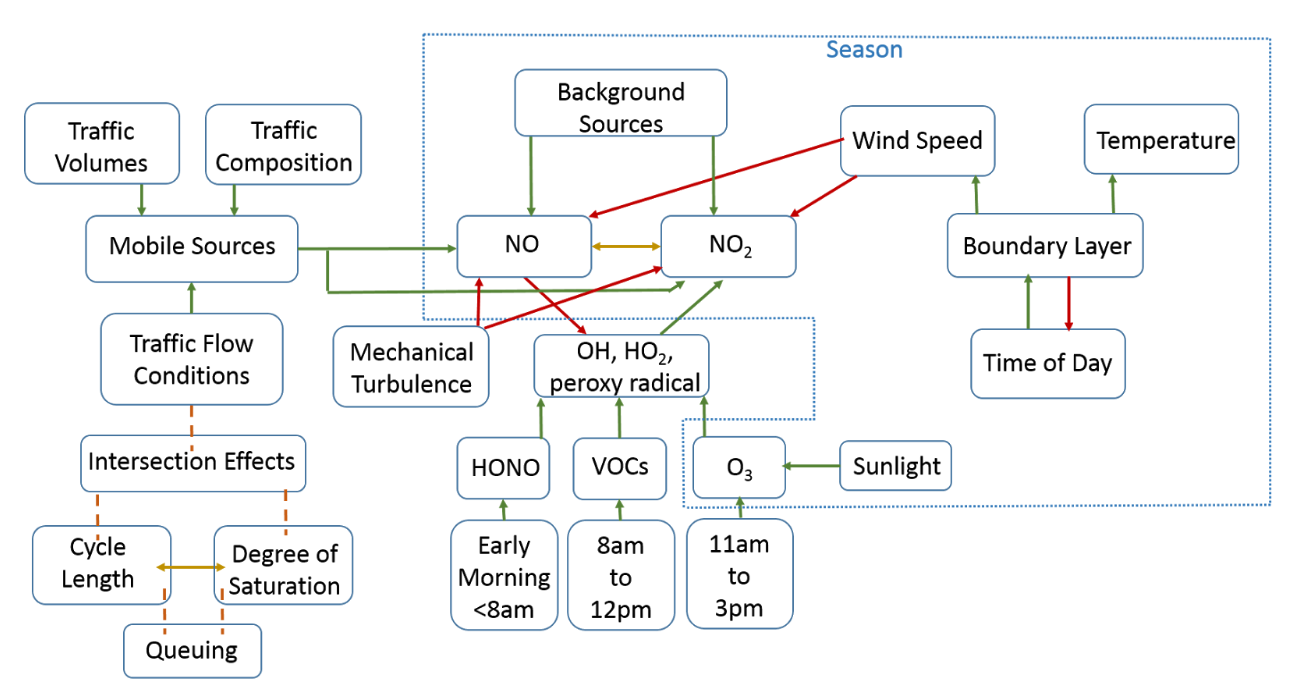
\includegraphics[width=\linewidth]{portland}
\end{figure}

The diagram correlates the system variables of an air pollution monitoring system with other, observable variables like traffic, the time of day, the presence of sunlight, and traffic. It presents an intuitive---and useful---description of the system at large.

Broadly, we want our diagrammatic calculus to have a notion of \emph{process}, \emph{state}, and \emph{effect}.

\begin{figure}[h!]
\centering

\includegraphics{process}
\end{figure}

Composition and tensoring of morphisms are represented, respectively, as below:
\begin{figure}[h!]
\centering
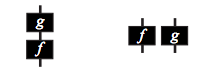
\includegraphics{composition}
\end{figure}

The reason we don't think about composition of correlations very much in a practical setting is because we almost always have direct data, and if we don't, we almost always do estimation of parameters and then use the learned model (e.g. Kalman filter or DBN) to estimate the correlation---the addition of using learned model means that you are always incurring a conditional [prior?] probability. When we use measurements, we are not invoking the underlying probabilities. Selling point: don't have to look at big collections of data. So all the different performance measures, we want to map them into a single grade e.g. 0-100. So to turn it into a single value or indicator.

% CHECK: does the correlation actually define a metric?

% Future work: we can also turn this into a supervised learning problem. We learn the correlations, present it to an expert, and ask is it right? Then the expert can sort groups into good and bad groups.

\section{Background}
Even within the constraints of a process theory, there are still a number of diagrammatic approaches to covariance. One, which we denote $\Rand$, defines the correlation as an inner product; another by \cite{coecke_spekkens} is $\Bayes$, which describes (perfect) correlation as a certain condition on a joint state.

The simplest approach, $\Rand$, uses the fact that real-valued, standard random variables over some fixed probability space $(\Omega, \mathcal{F}, \mathbb{P}$) form a Hilbert space where the inner product $\langle X, Y \rangle$ is just the covariance/correlation $E(XY)$. The objects of the category $\Rand$ are Hilbert spaces, morphisms are unitary matrices of the appropriate dimensions, composition $g \circ f : H \to H'$ is given by matrix multiplication, and the tensor is the matrix tensor product with unit $\mathbb{C}$. The states are normalized vectors representing probability distributions over the random variables.

With this setup, the correlation between two standard random variables (again, over the same probability space) is just the inner product in $(\Omega, \mathcal{F}, \mathbb{P})$, i.e. $\langle X, Y \rangle := \mathbb{E}(XY)$. It is depicted:
\begin{figure}[h!]
\centering
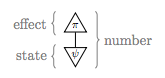
\includegraphics{innerproduct}
\end{figure}

\cite{coecke_spekkens} gives a similar graphical calculus for Bayesian inference. Restricting to standard probability, objects of the category $\Bayes$ are natural numbers, morphisms from $m$ to $n$ are $n \times m$ positive-valued matrices, composition is matrix product, and the monoidal product is the matrix tensor product. Normalized states are probability distributions over the set ${1, ..., n}$:

\begin{figure}[h!]
\label{bob_normalized_state}
\end{figure}

A joint state is a normalized state over the composite object ${1, ..., mn}$. A joint state is uncorrelated when it can be decomposed into a tensor product, and perfectly correlated when they are equal. So in $\Bayes$, a correlation is depicted:

\begin{figure}[h!]
\label{bob_uncorrelated_state}
\end{figure}

\begin{figure}[h!]
\label{bob_correlated_state}
\end{figure}

In \cite{lawvere}, the category of stochastic processes ...

Graphical models \cite{lauritzen} deal mostly with Markov processes and conditional dependence... 

$\Bayes$ and similar formalisms \cite{fong} give a semantics for \emph{causal} reasoning. Causal reasoning is useful for measuring the results of an experiment. It is not useful, generally speaking, when the data do not provide evidence for causation, such as in purely observational studies of complex systems. We want to carefully distinguish the causal aspects of our models from their non-causal aspects, and the first step is to develop a coherent framework for \emph{non-causal} reasoning. % more positive way of describing non-causal: what it means to have a status quo...

% \redout{A third approach fixes a specific Hilbert space of random variables and interprets it as a Lawvere metric space. But is there a monoidal product in this space? Even if not, and there is no graphical interpretation, would there still be a reason to do this?}

\section{Indicator Frameworks}
Before giving the definition of the category $\Ind$ of indicator frameworks, we will go through some of the statistical justification. Suppose that we have a correlation between $X$ and $Y$ and another one between $Y$ and $Z$. What can we say about the correlation between $X$ and $Z$? If we \emph{had} to guess, then the obvious guess would be 
\begin{equation}\label{eqn:guess1}\Cor(X,Y) = \Cor(X,Y)\Cor(Y,Z).\end{equation}
The following result is an exercise in \cite{?}.

\begin{lem}If $a = \Cor(X,Y)$ and $b = \Cor(Y,Z)$, then 
\begin{gather}
\Cor(X,Z) \geq ab - \sqrt{1-a^2}\sqrt{1-b^2} \\ 
\Cor(X,Z) \rangle \leq ab + \sqrt{1-a^2}\sqrt{1-b^2}
\end{gather}
\end{lem}

\begin{proof}
WLOG, assume that $A,B,C$ are standard variables with zero mean and unit variance, since the correlation is invariant under changes to mean and variance. We can write $X = a Y + O_Y^X$ and $Z = b Y + O_Y^Z$ where, by assumption, $O_Y^X, O_Y^Z$ are random variables uncorrelated with $Y$.

Then $\langle X, Z \rangle = \Cor(X,Z) = \langle aY + O_Y^X, bY + O_Y^Z \rangle = ab + \langle O_Y^X, O_Y^Z \rangle$.

We can use the Cauchy-Schwarz inequality to bound $\langle O_Y^X, O_Y^Z \rangle$ from above and from below, giving the lemma.
\end{proof}

The lemma tells us that there is a range of possible values for the composite correlation, depending on the values of component correlations. We can also interpret the range as a ``likelihood score'' on (\ref{eqn:guess1}). In the case where $\Cor(X,Y) = \Cor(Y,Z) = 1$, (\ref{eqn:guess1}) is most likely to be true; in the cases where one correlation is $-1$ and the other is 1, or when both are 0, (\ref{eqn:guess1}) is least likely to be true.

In such a situation, we may ask what is the obstruction to knowing the canonical or `true' composition---what, if we knew it, would tell us the true composition? We may simply ask for the data. Reading the proof, clearly what we need to know is the correlation $\langle O_Y^X, O_Y^Z \rangle$.

The natural product between random variables should be a tensor product.

Suppose we had some initial notion of how ``significant'' certain random variables was, relative to other variables.


Of course, we didn't have to derive this result to guess 

Now suppose that we have multiple correlations $\Cor(X,Y_i)$ and $\Cor(Y_i,Z)$. Can we say anything more about the correlation between $X$ and $Z$?

 for which we have correlations between $X$ and $Z$.
\[ \langle X , Z \rangle = \frac{1}{n} \sum_{i \in B}^n \langle X,Y_i \rangle \langle Y_i, Z \rangle.\] 
This assumes, however, that all the correlations are equally significant in supplying the correlation. Moreover, it fails to square with our intuition

\begin{define}The category $\Ind$ of indicator frameworks takes objects as finite-dimensional Hilbert spaces, morphisms from $V^m$ to $V^n$ as an $n \times m$ matrix of correlation coefficients, and composition as the correlation matrix generated by the following equation: 

\end{define}

\begin{lem}$\Ind$ is a symmetric monoidal category with tensor $\otimes$ and monoidal unit $\mathbb{C}$.
\end{lem}

Given this monoidal structure, a state is a [0,1]-valued vector in that Hilbert space, which is interpreted as a ``trustworthiness'' or ``prior'' vector on each of the indicators. An effect is interpreted as a ``priority'' vector on a (typically smaller) set of indicators.

In essence, the idea is to treat indicators as something closer to \emph{features} of a given optimization problem, rather than as random variables.

% We're probably going to have to introduce some method of measuring ``failure to correlate''.

% Alternately: correlation is the projection of one random variable (imagined as a vector) onto another random variable.

% This paper is the first in a series meant to articulate \emph{hybrid indicator frameworks}. The goals of this paper are (1) to give a graphical formalism for correlation, (2) to place the choice of `relevant' system variables in the context of a process theory, and (3) to say what it means for correlations to be verified by data obtained by `measuring' the system variables, and (4) to say what it means for correlations to verify or support causal models.

% [Justify the way we have defined this category in relation to what's already out there.]

% How can we add the statistical significance of the correlation to our model?

\section{Misc. Notes}
% \footnote{The reason for wanting a process theory of the variables represented in the correlation diagram is based on the intuition that each variable represents a functional component of a cyber-physical system, not a node in a network; this suggests a mathematical interpretation of the diagram should have more in common with the semantics of computation than with the modeling of complex networks.} 

Here are the things we'd like to model in our process theory:
\begin{enumerate}
\item Measurements of state
\item Correlations between indicators
\item General processes in the underlying complex system
\end{enumerate}

Continuing with the diagram. Some system variables may be measured, and we will refer to such measurable variables as \emph{indicators}.\footnote{The name `measurable variables' is confusing, since our notion of measurement is quite different from that of a measurable function or random variable.} Think of it like this: for every indicator, we have a specific technique or device that can be used to test for the physical state of that indicator. Arbitrary system variables in the complex system do \emph{not} have an assigned measurement device... but that doesn't mean they don't matter. 

When we measure an indicator, in principle we are always measuring change in the indicator, typically over time. Verifying a correlation requires, in principle, that we correlate the entire  There are some properties we expect of any measurement system, namely that we want to be able to analyze the data in certain ways. We certainly want to be able to measure change in the system.

But there is no underlying reality (state?) in the complex system. A state may not be measurable, but that doesn't mean it doesn't matter.

In our hypothetical category $\Ind$, what is a joint state, what is a product state, what is an entangled state? What is an effect, is there an inner product (i.e. are there adjoints?)? What are the scalars in the monoidal category? What is discarding?

\emph{For a given policy or project, what is the `right' set of indicators to measure it? Subtext: ``holistic''?} [Is this an optimization problem? In that case, we need to define a cost heuristic on (sets of) indicators. The problem is that ``indicators'' are not just numbers.]

We want to be able to define indicators from the top-down. A super-indicator is the ``goal'' from the Mayor's perspective, e.g. quality-of-life. We are trying to select the right sub-indicators to a super-indicator. And we are trying to present how to combine them.

Ultimate goal is very vague! The ultimate goal is sort of like a big integration over all these complicated things (both hands and eyes) that we have in hand. There's a feedback loop.

How do you formalize the method of quantifying the goals in any project or policy change? And we are providing a method in terms of `processes' and `measurements'.

A person has an ``intuitive sense of what they want''. We want to view this intuitive sense as just the decomposition rule into measurable things. This follows what a city person does in practice; they want to ``improve the transportation system''.

Is ``right'' defined just in terms of the projects or policies? Sort of; it's defined in terms of a super-indicator, some amorphous thing like ``quality of life'', which, for us, is defined partly in terms of the projects/policies ...!

Indicators as features: as components of a model.

Indicator is an outcome of the operation of a system.

You have state variables, but some of them are not observable because you can not measure them. So you use the measures that you can measure and observe, so that you can estimate the state. You have a state variable but you cannot observe it, so instead you use particular indicators.

Once you have a new policy, you want to identify the indicators that are affected.

A super-indicator is a ``conceptual'' indicator, which is NOT completely set down, and which is supposed to represent the priorities of the Mayor, and it should be definable, at least partly, in terms of the particular projects and policies. How do we contrast this with data-level indicators?

A super-indicator gives ``rules for decompositions''.

Method of constructing a cost function?





Cost functions can only be defined in terms of the 

Reverse of traditional optimization?

Not only their correlations, but also their contribution to some unspecified... 

What is an indicator (or a sensor)? It's a ``measurement tool''; alternately, you can think of it as a ``feature''; something that, given an input, outputs a 0 or a 1 depending on whether or not a stated effect has occurred. In the ONB formulation, it's a test for whether the input vector is equal to the stated effect.

What are the indicators measuring, i.e. what are the states? Unclear... 

What is time-series data from the indicator, i.e. what is data in this sense, and what notion of time? Since everything is relative, we're going to normalize 

We can think of data as the recorded values of the inputs and the outputs, but we can also think that ``data is just whatever it is that is used to output a model, i.e. a set of parameters''. So this is kind of

What is a ``cost function'' for some set of parameters?

What is an optimizer for a given cost function on the data? Clearly, something that iteratively minimizes the cost function over the parameters.





What is a policy or project? A process. What is evaluation or measurement? It is a 0,1 (or, possibly, something in [0,1] or, much more generally, a value in any symmetric monoidal category). What is a correlation? How do you deal with the fact that correlations in Set? 

Well, it seems that basically the problem is that instead of Hilbert spaces, where the cap between two states tests for equality (between basis states) and becomes just the inner product, we need to define some ``inner-product-like'' operation for 

Parameterized by the algebra (for aggregation of indicator values into other indicator values)

The end goal of this paper is to define a monoidal category for this diagrammatic calculus.

We introduce a diagrammatic calculus for reasoning about  Finally, we will define a monoidal category for this diagrammatic calculus.

``Knowledge about the indicators'' can be formalized through functors from other categories to the category of indicator frameworks.

\end{document}
